\section{Auditing the Cost Claims}\label{sec:cost}

The paper's Tables~II and~III give the repaired scheme exactly the same cost as Verma's scheme, and
its Figs.~3--5 plot those rows; its comparative claim, ``best efficiency'' among secure schemes, rests on
them~\cite{qiao2023}. The repaired verification equation \eqref{eq:qiao-verify}, however, has an extra
per-signer term $u_iR_i$ and an extra hash $H_2$ that Verma's \eqref{eq:verma-verify} does not. We
therefore counted the operations of the paper's own algorithms.

\subsection{Operation counts}\label{sec:cost-counts}
\prov{Ours}. \Cref{tab:counts} compares the printed rows with the counts measured by our instrumented
backend. The counts are identical on both backends and at every $n$ tested. Counted the same way, Verma's
scheme reproduces its printed rows exactly (except \textsf{Sign}, which omits one point addition), so the
method is sound and the discrepancy lies in the rows printed for the repaired scheme.

\begin{table}[ht]
\centering\small
\caption{Cost of the repaired scheme: printed in the paper vs counted from its algorithms.}\label{tab:counts}
\begin{tabular}{lll}
\toprule
Algorithm & Paper (Tables II--III) & Counted \\
\midrule
\textsf{Sign} & $1\Te+1\Th$ & $1\Te+2\Th$ \\
\textsf{Verify} (one signature) & $3\Te+2\Ta+2\Th$ & $4\Te+3\Ta+3\Th$ \\
\textsf{AggSign} & $(n-1)\Ta$ & no group operations ($n-1$ scalar additions) \\
\textsf{AggVerify} & $(n+2)\Te+(n+1)\Ta+2n\Th$ & $(2n+2)\Te+3n\Ta+3n\Th$ \\
\bottomrule
\end{tabular}
\end{table}

The \textsf{AggVerify} row printed for the repaired scheme is exactly Verma's row: one scalar
multiplication per signer where the equation needs two. Under the paper's own unit costs, at $n=100$, the
printed row evaluates to $12.729$~ms and the counted row to $25.324$~ms, a factor of $1.99$;
per signer, $0.125$ against $0.251$~ms. The value $12.729$~ms is exactly the bar the
paper plots for its scheme in Fig.~4, so that figure inherits the error. The paper also contradicts
itself: it charges scheme~[6] of its comparison (Verma \emph{et al.}'s PFCBAS) $(2n+2)\Te+(3n-1)\Ta+3n\Th$,
which at $n=100$ is $25.319$~ms, within one point addition of our count for the repaired scheme. One
row errs in the paper's favour: \textsf{AggSign} adds scalars, not points, so the printed $(n-1)\Ta$
overstates it.


\paragraph{Objections considered.}
(a)~\emph{Caching.} $h_0^i$ depends only on static values, so a verifier with a fixed roster can cache
it, removing $n$ hashes. Verma's $h_0^i$ is equally static, so the same caching lowers both schemes and
the difference remains. Caching the point $R_i+h_0^i\PTA$ per signer also reproduces the paper's printed
single-signature row, but the aggregate cost stays at $(2n+1)\Te$: $24.807$~ms at $n=100$, still
$\times1.95$. (b)~\emph{Algebraic folding.} $\sum u_iR_i+(\sum u_ih_0^i)\PTA=(\sum u_ic_i)P$ would be a
single multiplication, but $c_i$ is the signer's secret, so a verifier cannot use it. (c)~\emph{Multi-scalar
multiplication} is an optimisation, not what the tables count; \cref{sec:opt} examines it. A test pins
each of these arguments.

\subsection{Timing confirms the counts}
\prov{Experiment}. Counts are a model, so we also measured. The per-signer cost ratio of the repaired
scheme to Verma's is the slope ratio of aggregate verification time against $n$. The printed rows imply
a ratio of $1.00$; the counted rows predict about 2. Over 11 recorded runs on two curves and two machines
the measured ratio lies between $1.99$ and $2.48$ (\cref{fig:runs,fig:vsn}); \cref{tab:timing} gives the
medians.

\begin{table}[ht]
\centering\small
\caption{Measured per-signer cost ratio (repaired $\div$ Verma; median of runs), against the prediction
from operation counts priced with measured primitive costs.}\label{tab:timing}
\begin{tabular}{llccc}
\toprule
Machine & Curve / library & Runs & Measured & Predicted \\
\midrule
Ryzen 5 7520U & Ristretto255 / libsodium & 5 (3 used) & 2.153 & 2.143 \\
Ryzen 5 7520U & P-256 / OpenSSL & 5 (3 used) & 2.366 & 1.986 (2.363--2.371$^{\dagger}$) \\
Xeon 2.2\,GHz (Kaggle) & Ristretto255 / libsodium & 1 & 2.123 & 2.129 \\
\bottomrule
\end{tabular}

\smallskip
\footnotesize $^{\dagger}$ With each hash priced as the real call, including its point encodings
(\cref{sec:p256-gap}). Medians use the runs whose linear fit had $r^2\ge0.99$; all 11 runs lie in $1.99$--$2.48$.
\end{table}

\begin{figure}[ht]
\centering
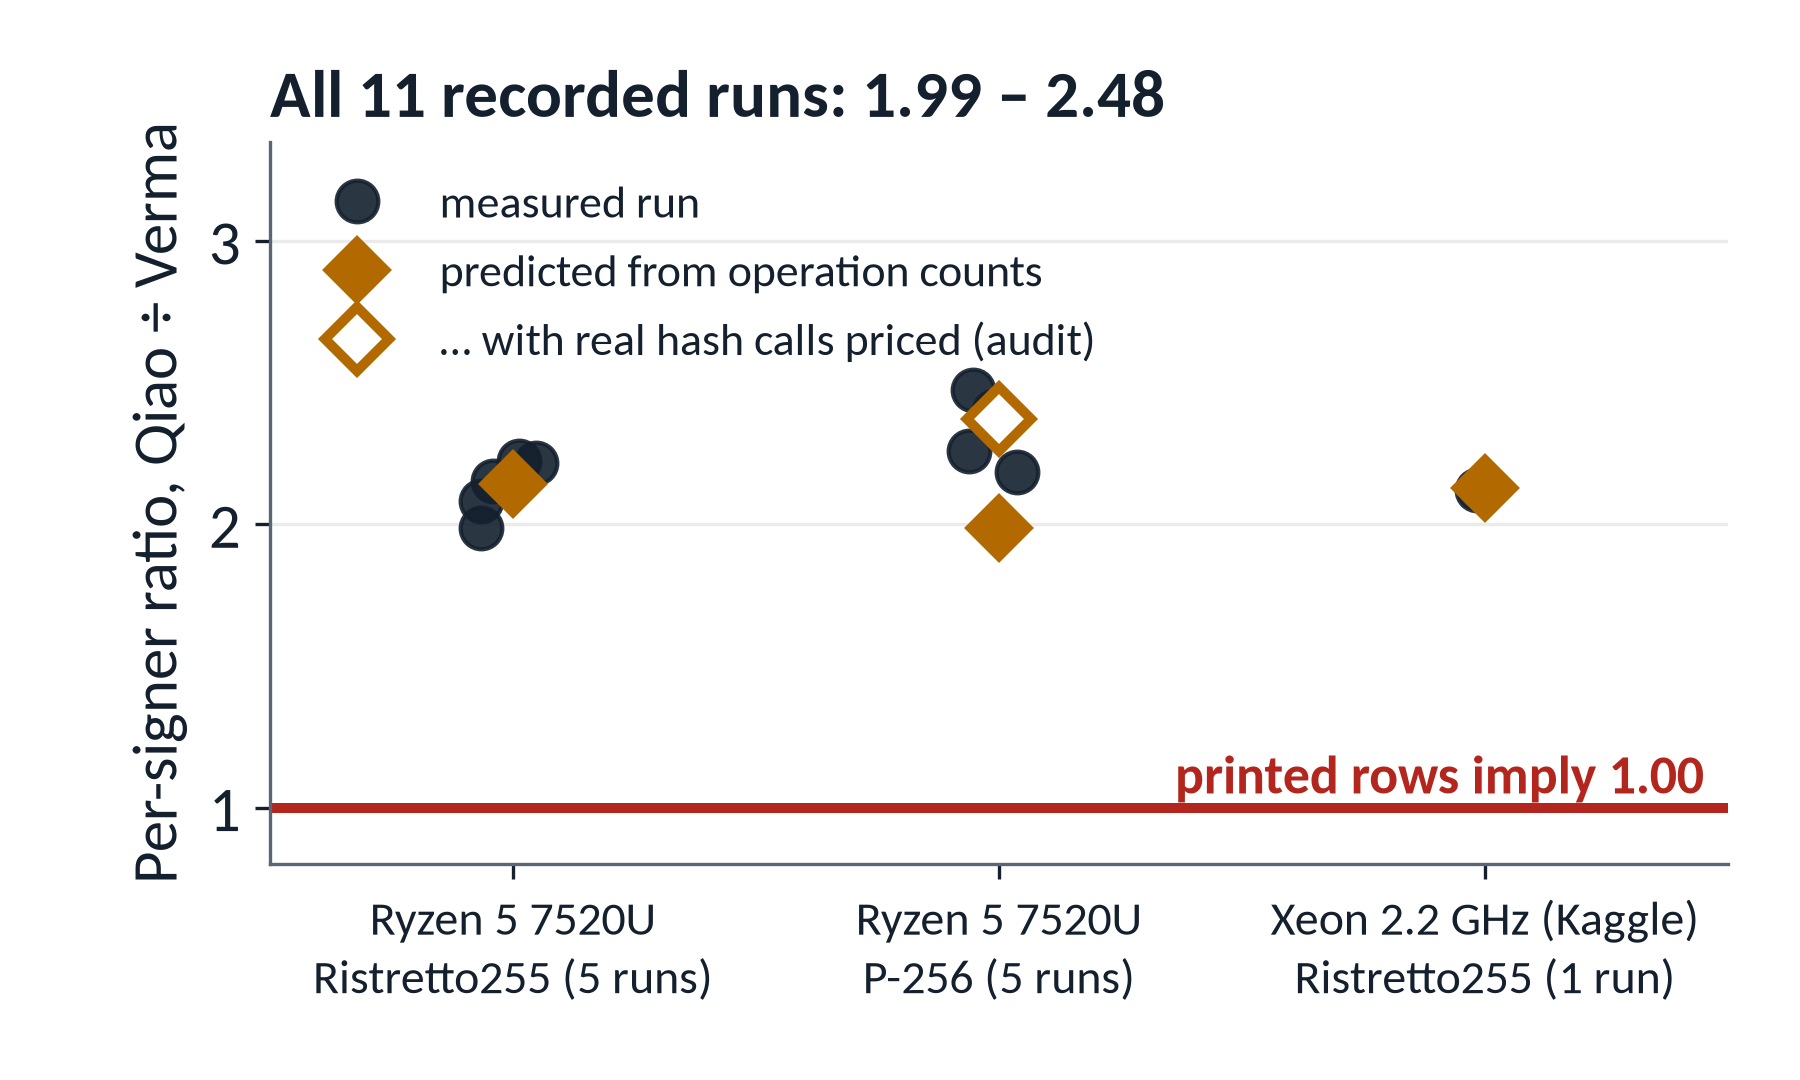
\includegraphics[width=0.74\linewidth]{figures/fig_ratio_runs.png}
\caption{Per-signer cost ratio (repaired $\div$ Verma) in all 11 recorded runs on two curves and two
machines, with the prediction from operation counts. The printed rows imply 1.00. Data:
\nolinkurl{bench/results/sweep_*.json}; the real-hash prediction comes from \code{make hashcost}.}
\label{fig:runs}
\end{figure}

\begin{figure}[ht]
\centering
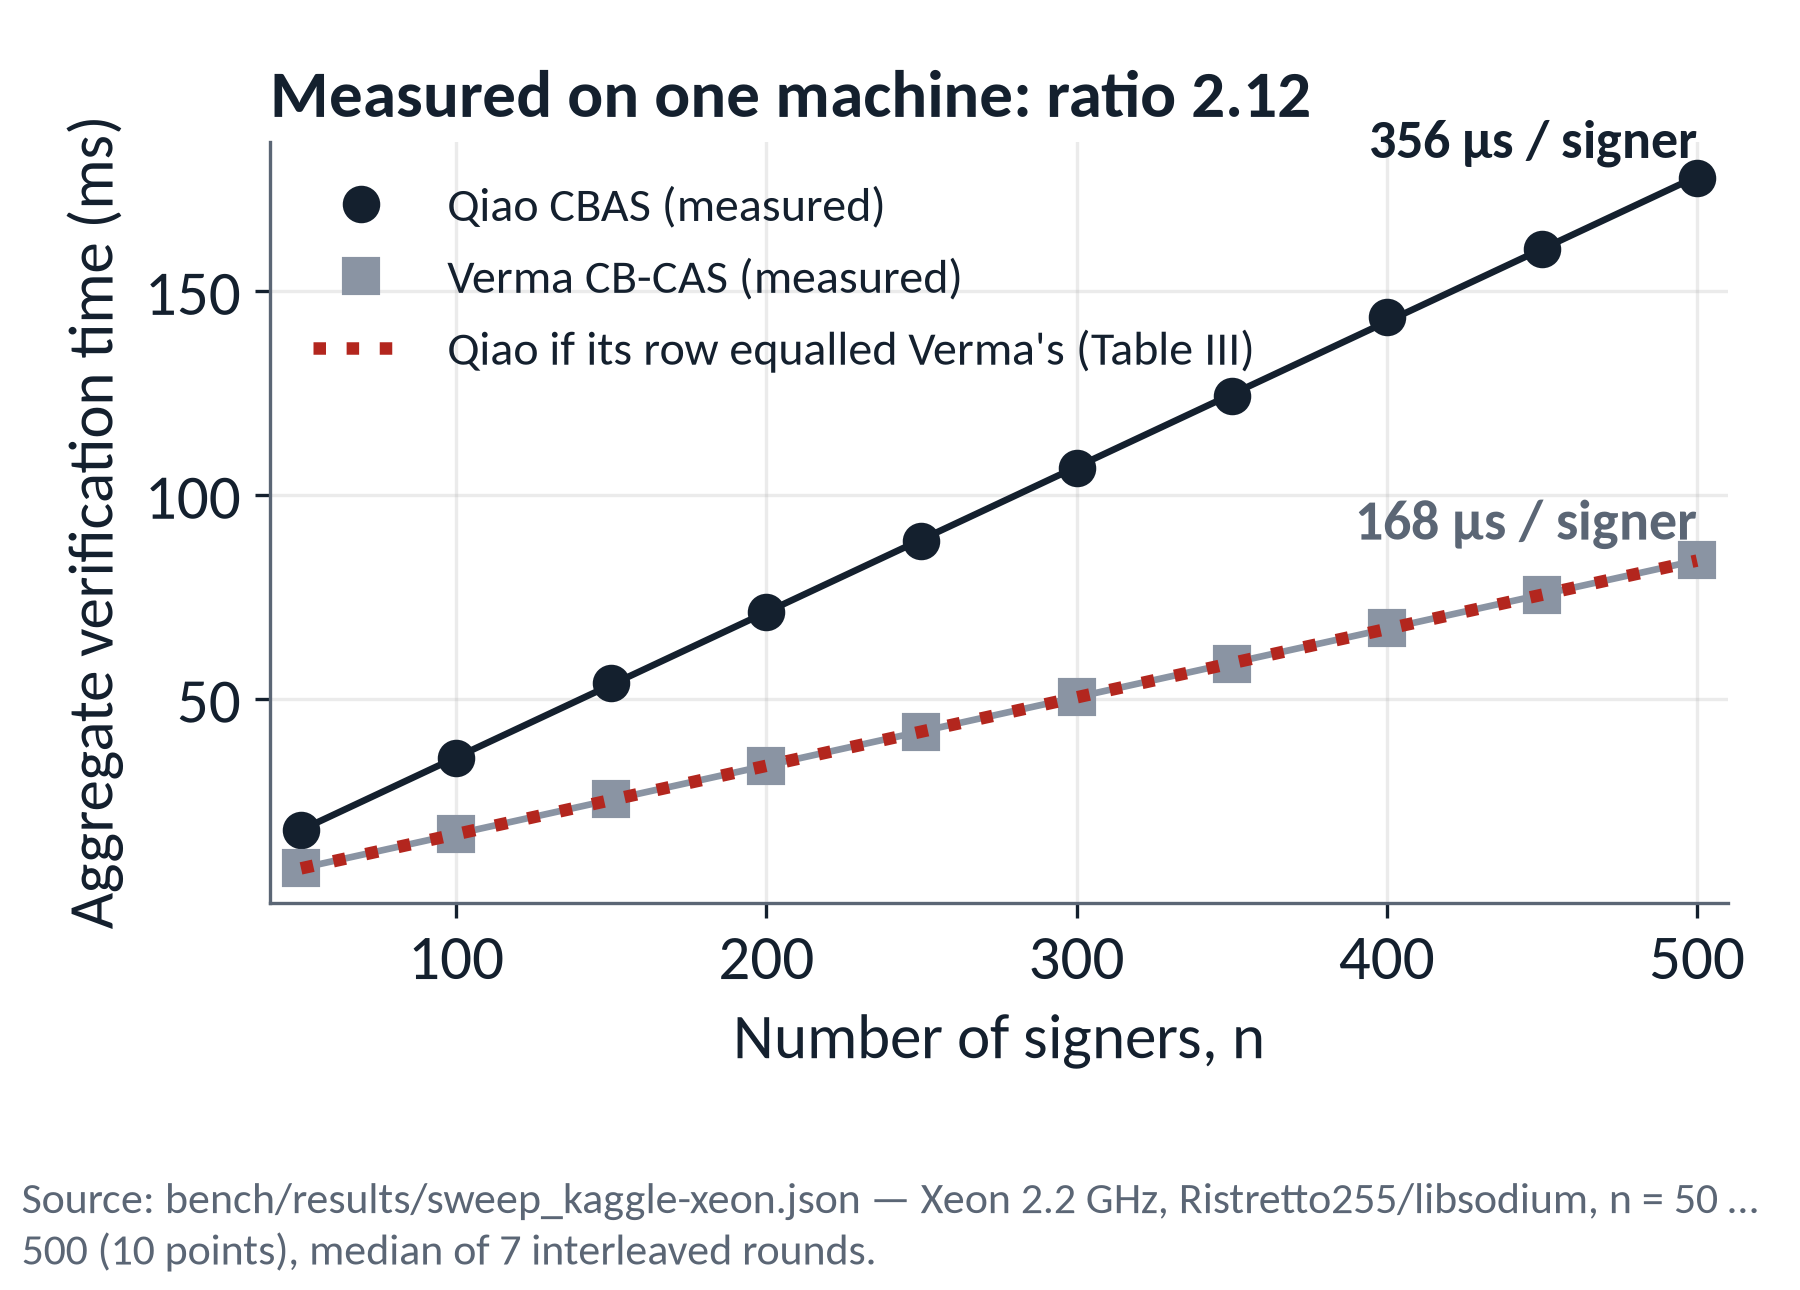
\includegraphics[width=0.74\linewidth]{figures/fig_measured_vs_n.png}
\caption{Aggregate verification time against $n$ on the second machine (Xeon, Ristretto255). The dotted
line is what the repaired scheme would cost if its row equalled Verma's.}
\label{fig:vsn}
\end{figure}

\subsection{Why P-256 timing exceeded the bare count}\label{sec:p256-gap}
On Ristretto255 prediction and measurement agree within $0.5\%$; on P-256 the measured ratio was about
20\% above the bare prediction. The cause is the cost of a real hash call. Each call serialises its point
arguments, and verification of the repaired scheme serialises 8 points per signer ($pk_i$ and $R_i$ in
$H_0$; $pk_i$, $R_i$ and $T_i$ in each of $H_1$ and $H_2$) against Verma's 2; a test counts them. In
OpenSSL a P-256 encoding costs a modular inversion, about twice a point addition, whereas libsodium stores
a Ristretto255 point as its encoding, making the same calls almost free. Pricing the real hash calls
predicts $2.363$--$2.371$ on P-256, against the measured $2.366$. The counts are therefore exact; the bare
model simply prices hashing too cheaply on one library.

\paragraph{Summary.} The paper's own equation costs about twice its printed row. This does not affect
the security of the construction; it affects the paper's efficiency comparison and the figures computed
from the tables.
